\chapter{ATTT và bảo mật hệ thống}
\label{ch:security}
\section{Mô hình đe dọa và phạm vi}
Tài sản cần bảo vệ gồm tài khoản quản trị, tác phẩm chờ duyệt, file ảnh, cấu hình kết nối và tính toàn vẹn website. Những đường vào chính là đăng nhập, upload, REST/wp-admin, endpoint WordPress và plugin. Đối tượng kiểm tra là website LocalWP do nhóm quản lý; không quét GitHub, website ngoài nhóm hay brute-force tài khoản thật. Kiểm thử local không mô phỏng đầy đủ TLS, reverse proxy và các đe dọa Internet của production.

Hardening giảm bề mặt và hậu quả của lỗi, còn vulnerability assessment thu thập dấu hiệu để đánh giá rủi ro. Chặn XML-RPC không chứng minh plugin không có lỗi; WAF chặn scanner không phải chứng minh mọi khai thác đều bị chặn. Báo cáo phân biệt rõ trạng thái plugin, cấu hình đã lưu và hành vi được xác nhận qua HTTP.\cite{wordpressSecurity}

\section{Bảo vệ tài khoản và khôi phục}
\subsection{URL đăng nhập và giới hạn thử sai}
WPS Hide Login chuyển endpoint đăng nhập bằng cơ chế WordPress hỗ trợ; không đổi tên vật lý wp-login.php/wp-admin. Liên kết đăng nhập, đăng xuất, quên mật khẩu và đích quay về upload được tạo qua API WordPress. Giá trị slug thật không nằm trong repo hay báo cáo. URL mới làm giảm request tự động vào endpoint mặc định, nhưng không phải yếu tố xác thực thứ hai và không thay mật khẩu mạnh.

LLAR là limiter đang phụ trách thử sai: 5 lần trong cửa sổ 900 giây, khóa 900 giây; 4 đợt khóa dẫn đến khoảng khóa dài hơn 3600 giây. Trên LocalWP, nhiều phiên có thể cùng hiện dưới loopback. Vì vậy test dùng tài khoản thử, chụp snapshot trạng thái limiter trước, không thử mật khẩu sai với tài khoản quản trị thật và phục hồi đúng snapshot sau test. Kiểm chứng cho thấy lần thứ năm bị khóa, mật khẩu đúng của tài khoản thử cũng bị từ chối trong thời gian khóa, rồi truy cập lại được sau thao tác phục hồi có kiểm soát.
\begin{figure}[H]\centering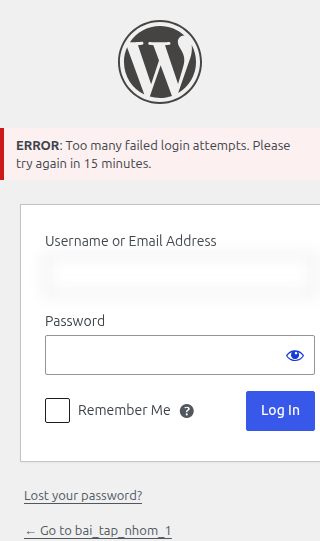
\includegraphics[width=0.38\linewidth,height=0.44\textheight,keepaspectratio]{figures/login-lockout.png}\caption[Khóa đăng nhập]{Ảnh khóa đăng nhập thật từ hồ sơ kiểm thử LocalWP; trường tài khoản đã che. Ảnh lịch sử được giữ cùng log hồi quy; không phải thử sai với admin thật.}\label{fig:lockout}\end{figure}

Khi quên URL, owner có thể dùng Site Shell lấy tùy chọn whl\_page hoặc vô hiệu riêng WPS Hide Login bằng CLI, sau đó cấu hình lại. Khi bị khóa, quản trị viên xác minh nguyên nhân và mở khóa qua CLI theo hướng dẫn, không đặt tác vụ tự xóa bộ đếm định kỳ. Nếu cần đổi tên thư mục plugin để phục hồi, chỉ đổi thư mục plugin; không đổi core. Khôi phục phải giữ phiên quản trị đang có hoặc đường CLI để tránh tự khóa người vận hành.

\subsection{Chính sách mật khẩu và Wordfence}
Module Lăng Kính Security kiểm tra mật khẩu mới/đổi ở hồ sơ, reset và REST: tối thiểu 12 ký tự, chữ hoa, thường, số, ký tự đặc biệt; từ chối một số chuỗi phổ biến. Không tự đổi mật khẩu quản trị hiện hữu. Kiểm tra ở REST callback boundary trả WP\_Error trước khi cập nhật; việc đặt error sai loại vào filter chuẩn bị object là một lỗi từng được sửa. Đường CLI/programmatic tin cậy được giữ để khôi phục, nên không tuyên bố mọi plugin gọi trực tiếp API PHP đều chịu cùng policy.

Wordfence 9.0.2 đang active, có key và onboarding hoàn tất; WAF ở Enabled/Basic Protection. Basic chạy trong bối cảnh WordPress, không được gọi là Extended Protection. Hai thành phần login/password tương ứng của Wordfence được tắt để tránh trùng với LLAR/module. Cần phân biệt key hiện diện với giấy phép trả phí: báo cáo không có bằng chứng quyền sử dụng Premium và không nhận là đã quét malware đầy đủ.\cite{wordfence}

\section{Hardening ứng dụng và máy chủ}
Module bảo mật tách khỏi theme để chính sách không biến mất khi đổi giao diện. Các hook loại generator HTML/feed, bỏ X-Pingback, thêm nosniff và referrer policy, từ chối XML-RPC ở lớp WordPress và vô hiệu file editor. Việc ẩn generator chỉ giảm một nguồn fingerprint; query ver của tài nguyên vẫn được giữ để cache busting. Header router LocalWP có thể còn báo phiên bản Nginx, vì thế không tuyên bố đã giấu toàn bộ dấu vết công nghệ.
\shot{hardening-current.png}{Màn hình Lăng Kính Security trên LocalWP trong đợt bàn giao. Nguồn: ảnh chụp mới bằng tài khoản thử; đây là trạng thái cấu hình, hành vi còn được kiểm tra bằng HTTP.}{fig:hardening}

Nginx có \code{autoindex off} và exact location chặn XML-RPC, readme, wp-config, trình cài đặt/setup không cần sau cài. Rule đặt trong template \code{conf/nginx/...hbs}, không chỉ .htaccess và không chỉ runtime. PHP tắt display\_errors, display\_startup\_errors, expose\_php, giữ log\_errors. Sau Stop/Start phải so lại runtime và status HTTP; một rule trong repo chưa triển khai không phải bằng chứng site đã được hardening.

Quyền thư mục/file được áp dụng trong application root sau khi xác minh owner và tài khoản chạy dịch vụ. wp-config thực tế là 400, PHP vẫn đọc được; thư mục 755, file ứng dụng 644, dữ liệu Wordfence có file 600. Plugin tạo file mới có thể chịu umask riêng, cần theo dõi derivative. LocalWP từng tạo helper debug rộng hơn sau Start; module chỉ sửa đúng helper trong môi trường local, không chmod toàn home. Upload và watermark được chạy lại để kiểm tra không bị hỏng do quyền.

\begin{table}[H]\centering\small
\caption{Đối chiếu trạng thái, cấu hình và hành vi bảo mật}
\begin{tabularx}{\linewidth}{lYYY}\toprule Thành phần & Đã bật/lưu & Kiểm chứng hành vi & Giới hạn\\\midrule
WPS Hide Login & Active, slug riêng & Login/logout và quay về upload & Không thay xác thực đa yếu tố.\\
LLAR & 5 lần / 15 phút & Khóa lần 5, phục hồi truy cập & IP local dùng chung; test đã hoàn nguyên bộ đếm.\\
Policy mật khẩu & Module active & REST/profile từ chối yếu; reset có log lịch sử & Không ép đổi mật khẩu cũ; CLI là đường tin cậy.\\
Nginx hardening & Template + runtime & XML-RPC và thư mục trả 403 & Không đại diện cho cấu hình router production.\\
Wordfence & Enabled/Basic, có key & Scanner UA mặc định từng bị 403 & Không chứng minh Extended, Premium hay malware scan.\\\bottomrule\end{tabularx}
\end{table}

\section{Đánh giá lỗ hổng và lịch sử WPScan}
\subsection{Nguồn dữ liệu và các lần chạy}
Hồ sơ có các lần WPScan 3.8.28 không token do công cụ chạy trước đây, một lần bị WAF chặn và lần Docker 4.1.0 có API do người dùng cung cấp. Không gộp các log thành một lần quét mới. Bản 4.1.0 báo Started/Finished ngày 27/10/2026 nhưng console không in timezone; không tự quy đổi thời gian đó thành UTC. Các mốc UTC của 3.8.28 lấy từ trường timestamp trong JSON.

\begin{longtable}{P{3.2cm}P{4.6cm}P{6.7cm}}
\caption{Các lần WPScan và giới hạn đọc kết quả}\label{tab:scans}\\\toprule Lần chạy & Số liệu & Diễn giải\\\midrule\endfirsthead\toprule Lần chạy & Số liệu & Diễn giải\\\midrule\endhead
3.8.28 trước & 09:14:45--09:16:22 UTC; 690 request, 11 cache & Không có vulnerability API. Exit 0 ghi trong hồ sơ cũ; sanitizer cũ từng suy mã thoát nên cần runner gốc nếu tái xác minh exit.\\
3.8.28 bị chặn & UA mặc định; HTTP 403; hồ sơ ghi exit 4 & Scan aborted; không coi là scan sạch hay hoàn tất.\\
3.8.28 retry sau & 10:43:31--10:45:26 UTC; 712 request, cache 0 & Random UA, không tắt WAF. Không có API; không suy WAF Enabled chỉ từ UA.\\
Docker 4.1.0 & 12:18:16--12:18:24 theo console; 15 request, 9 cache & Người dùng thực hiện. API Free OK, dùng 3, còn 19; exit không được capture độc lập qua pipeline tee.\\\bottomrule
\end{longtable}

Lệnh Docker được trình bày bỏ token thực và không chứa login riêng:
\begin{Verbatim}[fontsize=\scriptsize,breaklines=true]
docker run --rm --network host \
  --add-host=baitapnhom1.local:127.0.0.1 \
  -e WPSCAN_API_TOKEN wpscanteam/wpscan \
  --url http://baitapnhom1.local --random-user-agent \
  --enumerate vp,vt --detection-mode passive \
  --plugins-detection passive
\end{Verbatim}
Token phải được truyền bằng cơ chế riêng trên máy, không chép giá trị vào lệnh lưu Git. Muốn lưu exit thật của pipeline Bash cần lấy PIPESTATUS của WPScan ngay sau pipeline, hoặc dùng runner subprocess.returncode. Mã thoát tee không đại diện mã thoát scanner.\cite{wpscan}

Docker retry không nhận diện phiên bản core, không phát hiện plugin bằng passive và nhận diện Astra 4.14.1 với confidence 80\%. ``No plugins Found'' không có nghĩa site không cài plugin. Inventory filesystem xác nhận các plugin thực tế, nên đánh giá độ phủ phải đối chiếu cả hai nguồn. Metadata WPScan lúc đó ghi latest Astra 4.14.0 trong khi nhận diện 4.14.1; không tự hạ cấp theme hoặc tự gán lỗi từ bất nhất metadata.

\subsection{Bảng đánh giá có căn cứ}
\begingroup\small\setlength{\tabcolsep}{3pt}
\begin{longtable}{P{2.4cm}P{3.2cm}P{1.4cm}P{2.3cm}P{2.7cm}P{2.6cm}}
\caption{Cảnh báo cấu hình, bằng chứng và xử lý}\label{tab:assessment}\\\toprule Phát hiện & Bằng chứng & Lớp & Mức/căn cứ & Khắc phục & Sau xử lý\\\midrule\endfirsthead\toprule Phát hiện & Bằng chứng & Lớp & Mức/căn cứ & Khắc phục & Sau xử lý\\\midrule\endhead
Author tự publish & REST từng trả 201 publish & Theme & High đối với quy trình duyệt; không gán CVE & CPT capability riêng, migration & REST 403; wp-admin không publish.\\
XML-RPC mở & Trước GET 405, scanner thấy endpoint & Server / core & Medium: RPC không dùng, mở bề mặt auth & Nginx 403 + module fallback & Sau Stop/Start vẫn 403.\\
Quyền config rộng & Hồ sơ baseline 664, root 775 & Server & Medium: có thể lộ DB secret cho user local & Root 755, file 644, config 400 & PHP đọc được, upload thành công.\\
Thiếu limiter/policy & Inventory và test baseline & Plugin / auth & Medium: thiếu lớp giảm thử sai & LLAR + policy module & Khóa lần 5; REST/profile yếu bị chặn.\\
Generator / readme & HTML/feed và phát hiện scanner trước & Core / server & Low: nhận diện, chưa có exploit & Hook generator, chặn endpoint & Feed/meta mất generator; ver CSS/JS giữ.\\
Directory browsing & Baseline đã 403 & Server & Thông tin; phòng ngừa & autoindex off tường minh & HTTP vẫn 403; không khẳng định từng lộ listing.\\
WAF chỉ Basic & Trạng thái cấu hình firewall & Plugin & Thông tin: giới hạn chế độ & Giữ Basic, không sửa vendor & Không tuyên bố Extended.\\
Server header & Router vẫn có thể lộ nginx & Server & Low: hỗ trợ nhận diện & server\_tokens site, tắt expose PHP & Chưa ẩn mọi header router.\\
API / coverage thiếu & 3.8.28 thiếu token; Docker passive trống & Quy trình & Medium về thiếu bằng chứng, không phải CVE & Đối chiếu từng slug/version với dữ liệu cập nhật & API OK chưa đủ phủ toàn inventory.\\
Pass Thru theme & 200 HTML, body rỗng; JPG mở được & Plugin / server & Thông tin: lỗi chức năng, không phải CVE & Rewrite Nginx + WebP marked & WebP/fallback HTTP đúng.\\\bottomrule
\end{longtable}\endgroup

Mức trong bảng thể hiện rủi ro trong bối cảnh ứng dụng hoặc cấu hình, không phải điểm CVSS tự tính. Không có bằng chứng xác nhận khai thác CVE hoặc xâm nhập trong phạm vi này. Robots/WP-Cron là endpoint tiêu chuẩn từng được tool liệt kê; chưa có bằng chứng DoS nên không tắt bừa, tránh hỏng scheduler/chuyển ảnh.

\subsection{Sanitizer, bảo vệ log và giới hạn còn lại}
Sanitizer hiện yêu cầu tool version, argv, exit thực và SHA-256 raw trong metadata đã xác minh. Input rỗng/sai schema bị từ chối; exit thiếu ghi unknown; scan aborted tách riêng. Timestamp giữ theo raw, không đổi thời gian chạy cũ thành thời điểm biên soạn báo cáo. Random user-agent không được dùng để suy trạng thái WAF. Các báo cáo lịch sử được giữ nguyên và có chú thích về giới hạn công cụ cũ, không tái tạo metadata giả.

Trong đợt bàn giao phát hiện regex che Authorization cũ có thể chỉ che chữ Bearer rồi để lại credential. Bản sửa che toàn bộ giá trị header Authorization/Proxy-Authorization/Cookie trên dòng đó. Test gồm Bearer, Basic, Negotiate, cookie nhiều phần và kiểm tra dòng Server tiếp theo còn nguyên. Đây là test tổng hợp bảo vệ tính riêng tư của script, không phải bằng chứng đã khai thác token thật. Chín nhóm test sanitizer đã qua trước khi xuất dữ liệu mới.

Không có ảnh console WPScan mới được dựng lại từ text để giả một lần chạy. Console retry thật dạng text và JSON đối chiếu được dẫn ở hồ sơ repo. Nếu cần ảnh toàn cửa sổ terminal do giảng viên yêu cầu, người quản lý cần chụp lần chạy thật hoặc mở log lịch sử với nhãn rõ ràng, che host/token. Không có kết quả ZAP/Nmap, không có pentest Internet, và không kết luận ``không có lỗ hổng'' từ passive scan thiếu độ phủ API.

\section{Lập trình an toàn và hồi quy}
Sanitization dùng đúng ngữ cảnh nhập: text cho tiêu đề/choice, textarea cho mô tả; validation xác nhận term thuộc taxonomy, giới hạn độ dài, upload error và MIME thực. Khi dựng HTML dùng esc\_html, esc\_attr, esc\_url, esc\_textarea. Nonce chống CSRF đi cùng capability; nonce đơn lẻ không cấp quyền. WordPress xử lý truy vấn/lưu bài qua API thay vì ghép SQL từ request.

Hai đoạn ngắn sau lấy trực tiếp từ handler hiện tại, thể hiện quyền và nonce là hai kiểm tra độc lập; đây là trích đoạn, không phải toàn bộ hàm:
\sourcefile{astra-child/inc/upload-form.php}{77}{80}
\sourcefile{astra-child/inc/upload-form.php}{97}{103}

Request upload chỉ tạo dữ liệu sau kiểm tra cần thiết; trạng thái pending được đặt server-side. Quyền riêng CPT còn bảo vệ qua REST/wp-admin nên một trường status giả không vượt kiểm duyệt. Lỗi lưu có cleanup và lỗi quá POST-limit nhận thông báo thay vì thành công giả. Đầu ra thông báo được escape, không đưa tên file độc hại vào HTML thô.

\begin{table}[H]\centering\small
\caption{Kết quả kiểm thử và mức bằng chứng}
\begin{tabularx}{\linewidth}{YYl}\toprule Nhóm kiểm tra & Kết quả quan sát & Trạng thái\\\midrule
Upload / duyệt & Hai ID pending; Editor publish; Author bị từ chối publish & Passed LocalWP\\
Input không hợp lệ & Guest/thiếu quyền, nonce sai, JPEG giả, 13 MB bị từ chối & Passed LocalWP\\
POST-limit & 17 MB vượt PHP tạm 16 MB, HTTP 413; đã khôi phục template & Passed đợt sửa lỗi\\
WebP và UI & MIME/Vary/body; watermark; filter/search/album/lightbox/mobile & Passed LocalWP\\
Login/hardening & URL riêng, logout, lần sai thứ 5, XML-RPC/directory 403 & Passed LocalWP\\
SQL restore & Import DB thứ hai; media, taxonomy, serialized data, admin mới & Passed môi trường riêng\\
Sanitizer & 9 nhóm test schema/exit/API/redaction/metadata & Passed tổng hợp\\
CVE toàn inventory & Chưa có dữ liệu API đối chiếu đủ từng thành phần & Chưa xác minh\\
ZAP/Nmap/production & Không thực hiện trong phạm vi & Unrun\\\bottomrule\end{tabularx}
\end{table}

Không phát hiện lỗi JavaScript ngoài dự kiến trong lượt hồi quy; kiểm tra cú pháp PHP/JS qua. Dữ liệu thử dùng tài khoản dùng một lần và được dọn; hash tác phẩm gốc, thumbnail, mật khẩu và theme mods được so để phát hiện thay đổi ngoài phạm vi. Kiểm thử không chứng minh mọi thiết bị/trình duyệt hoặc mọi định dạng ảnh đều không có lỗi. Những hạn chế đó cần đi cùng kết quả passed để người nhận hiểu đúng mức bảo đảm.
